\documentclass[12pt, a4paper, twoside]{book}
\usepackage[utf8]{inputenc}
\usepackage[english, serbianc]{babel}
\usepackage{lipsum}
\usepackage{graphicx}

\usepackage{geometry}
\geometry{
	a4paper,
	total={160mm,237mm},
	left=30mm,
	top=30mm,
}

\usepackage{hyperref}
\usepackage{xcolor}
\hypersetup{
	colorlinks,
	linkcolor={red!50!black},
	citecolor={blue!50!black},
	urlcolor={blue!80!black}
}

\usepackage{fancyhdr}
\pagestyle{fancy}
\fancyhead{}
\fancyhead[RE]{\leftmark}
\fancyhead[LO]{\rightmark}
\fancyfoot{}
\fancyhead[LE, RO]{\thepage}

\usepackage{amsmath}
\usepackage{amsthm}
\numberwithin{equation}{section}
\newtheorem{theorem}{Теорема}
\newtheorem{definition}{Дефиниција}

\begin{document}
\begin{titlepage}
	\newcommand{\HRule}{\rule{\linewidth}{0.5mm}}
	\center
	
	\textbf{\LARGE УНИВЕРЗИТЕТ У БЕОГРАДУ\\MАТЕМАТИЧКИ ФАКУЛТЕТ}
	\begin{figure}[!ht]
		\centering
		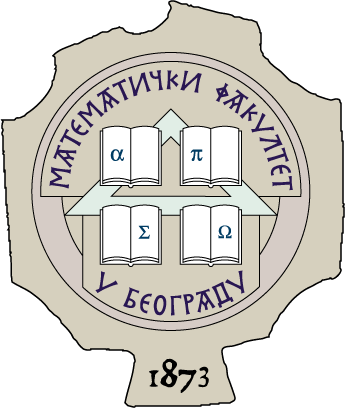
\includegraphics[width=0.2\textwidth]{img/matf-logo.png}
	\end{figure}\\[3cm]
	\textbf{\Large МАСТЕР РАД}\\[0.3cm]
	на катедри за \\[0.3cm]
	\textbf{\Large Рачунарство и информатику}\\[.7cm] % Minor heading such as course title
	на тему\\[0.7cm]
	
	\HRule \\[0.4cm]
	{ \huge \bfseries Примена неуронских поља зрачења у рендеровању}\\[0.4cm] % Title of your document
	\HRule \\[1.5cm]
	
	\begin{minipage}{0.4\textwidth}
		\begin{center}
			Коста Грујчић
		\end{center}
	\end{minipage}\\[5cm]
	
	{\large Београд, \today}\\[2.5cm]
	\vfill
\end{titlepage}
\pagenumbering{roman}

% Defines mentor & date
\newpage
\thispagestyle{empty}

\hspace{0pt}
\vfill
\noindent \textbf{Ментор}:\\
проф. др Младен Николић\\Универзитет у Београду, Математички факултет
\\[2cm]

\noindent \textbf{Чланови комисије}:
\\проф. др Младен Николић\\Универзитет у Београду, Математички факултет
\\[0.25cm]
\\проф. др Младен Николић\\Универзитет у Београду, Математички факултет
\\[0.25cm]
\\проф. др Младен Николић\\Универзитет у Београду, Математички факултет
\\[2cm]

\noindent \textbf{Датум одбране}: \today
\hspace{0pt}
\vfill

\newpage
\thispagestyle{empty}
Посвета

\newpage
\thispagestyle{empty}
\noindent \textbf{Наслов мастер рада}: Примена неуронских поља зрачења у рендеровању

\noindent \textbf{Резиме}:

\noindent \textbf{Кључне речи}: машинско учење, неуронска поља, рендеровање

\listoffigures
\listoftables
\tableofcontents

\pagenumbering{arabic}
\chapter{Увод}
\lipsum[1-20]

\chapter{Основни појмови рачунарске графике}
\section{Светлост}
\section{Камера}
	\begin{theorem}
		Неки текст теореме.
	\end{theorem}
	\begin{proof}
		Доказ теореме.
	\end{proof}
	\begin{definition}
		Неки текст дефиниције.
	\end{definition}
	\begin{equation}
		\int_{-\infty}^{\infty}f(t)dt
	\end{equation}
\section{Рендеровање}

\chapter{Основни појмови машинског учења}
\lipsum[1-20]

\chapter{Неуронска поља зрачења}
\section{NeRF}
\lipsum[1-10]
\section{Mip-NeRF}
\lipsum{1-10}
\section{Instant-NGP}
\lipsum[1-10]

\chapter{Скупови података}
\lipsum[1-20]

\chapter{Експерименти}
\section{Време обучавања}
\section{Квалитет резултата}

\chapter{Закључак}

\end{document}
